\chapter{Introduzione}
\label{chap:intro}
\section{Sommario}
Qui di seguito sono riportati i concetti fondamentali trattati all'interno del documento
\subsection{Informazione e segnali}
\label{sec:Informazioneesegnali}
L'informazione sussiste solo se il ricevente della trasmissione non conosce il
contenuto della suddetta.\\ Per esistere una trasmissione devono esserci:
\begin{enumerate}
  \item Comunicazione;
  \item Mezzo di trasmissione;
  \item Informazione.
\end{enumerate}

\subsection{Informazioni analogiche e digitali}
\label{sec:andiginfo}
Visto che è un argomento riccorrente all'interno del programma è giusto dare quanto
meno, una definizione anche se stringata, quindi:
\begin{defi}
  \label{def:andef}
  si dicono grandezze analogiche quelle che possono assumere tutti i valori
  intermedi all'interno di un dato intervallo; Si dicono grandezze digitali
  quelle che vengono espresse in modo numerico, senza possibilità di
  discriminare valori intermedi tra due cifre consecutive.
  Ulteriori approfondimenti presenti in (\ref{sec:sanalog})
  \footnote{\href{https://it.wikipedia.org/wiki/Analogico}{https://it.wikipedia.org/wiki/Analogico}}
\end{defi}
\begin{defi}
  \label{def:digdef}
  Con digitale o numerico, in informatica ed elettronica, ci si riferisce a tutto ciò che
  viene rappresentato con numeri o che opera manipolando numeri, contrapposto all'analogico. Ulteriori approfondimenti presenti in (\ref{sec:sdigital})
  \footnote{\href{https://it.wikipedia.org/wiki/Digitale_(informatica)}{https://it.wikipedia.org/wiki/Digitale\_(informatica)}}
\end{defi}
\begin{oss}
  \label{oss:strumMisura}
  Tipicamente quando si tratta di strumenti di misurazione entrambi i tipi di
  informazione entrano in gioco per poter funzionare. Ad esempio una sonda per
  un formo prende in ingresso in informazione analogica ``la temperature'' e poi
  la converte tramite l'apposito ADC a un informazione digitale per poterla
  campianare ed elaborare tarmite una centralina di gestione. 
\end{oss}
Oggi ormai utilizziamo il digitale perché effettivamente i calcolatori
elettronici gestiscono meglio una codifica rispetto a dei numeri reali. Per di
più costa meno produrre un dispositivo che gestisca segnali digitali rispetto
ad un dispositivo che gestisce mezzi analogici.
Ad esempio la differenza tra lo standard VHS e lo standard CD/DVD/Blue Ray, infatti,
il VHS era uno standard basato su un nastro magnetico, cosa che negli ultimi suoi anni
di vita si mescolò anche con il digitale ma uno dei limiti veri restava proprio il
supporto fisico, infatti, il nastro magnetico è molto fragile e incline ad avere
tantissimi problemi anche di prestazioni in utilizzi di archiviazione dati.
\subsection{Alcune osservazioni}
\begin{itemize}
\item Non tutte le informazioni costituiscono un vero e proprio contenuto
  inforamtivo
  \begin{enumerate}
  \item La notizia comunicata deve per noi essere eclatante;
  \item una persona noiosa non apporta informazione perché ripete
    continuamente gli stessi argomenti.
  \end{enumerate}
\item Problema di misurazione del contenuto informativo
  \begin{itemize}
  \item {\bf Claude E. Shannon} ({\tt 1916-2001}), fondatore della
    \textit{Teoria Matematica dell'Informazione}, è stato il primo
    ad introdurre la distinzione tra forma e significato nel
    processo comunicativo.
  \end{itemize}
\end{itemize}
\subsubsection{I risultati di Shannon}
\begin{itemize}
	\item Non è possibile definire la quantità di informazione associata ad un
		messaggio già ricevuto, ma piuttosto la quantità di informazione
		associata ad un papabile messaggio
		\begin{itemize}
			\item \textit{``information is that which reduces uncertainty''}
		\end{itemize}
	\item La quantità di informazione associata ad un massaggio è tanto più
		altra quanto più esso è inatteso
		\begin{itemize}
			\item il messaggio ``{\bf domani sorgerà il sole}'' ha un bassissimo
				contenuto informativo perché è assolutamente scontato e banale
			\item il messaggio ``{\bf Domani scoppierà la guerra}'' ha un alto
				contenuto informativo.
		\end{itemize}
\end{itemize}
\section{I segnali}
\begin{itemize}
	\item \textit{Grandezze fisiche variabili nel tempo a cui è associata
		un'informazione};
	\item \textit{L'informazione è associata ad una variazione ({\color{red}
		aleatorio} e non deterministica) della grandezza fisica};
	\item Aleatorio (dal latino ``alea'', gioco di dati) è sinonimo di non
		predicibile a priori (in contrapposizione con deterministico).
\end{itemize}
\subsection{Rappresentazione dell'informazione}
\label{sec:rappredellinfo}
\begin{itemize}
\item Associazione tra caratteristiche (di valore e temporali) dei segnali
  e le informazioni che essi rappresentano;
\item Le caratteristiche sono impresse dal dispositivo generatore del
  segnale;
\item Quali caratteristiche?
  \begin{itemize}
  \item valore, andamento temporale ed eventi del segnale (es.
    superare una soglia), etc.
  \end{itemize}
\end{itemize}
\subsection{Classificazione di segnali}
\label{sec:classsegn}
I segnali vengono classificati in base alla loro natura e alle loro caratteristiche.
Tipicamente per il campionamento avviene il seguente processo:
\begin{center}
  Grandezza fisica \textrightarrow{} trasduttore \textrightarrow{} segnale elettrico 
\end{center}
Quindi prendendo come base questa affermazione, possiamo dire che un segnale che sia
di natura elettrica, acustica o qualunque altra natura fisica, può essere campionato
da uno strumento che tramite il suo trasduttore converdirà in un istruzione
``tipicamente definita pacchetto di istruzioni o di informazioni'' che a sua volta
verrà convertito in un segnale elettrico che seguendo lo standard di comunicazione
del modello\footnote{una variazione della corrente elettrica o di tensione all'interno
  di un conduttore oppure in un punto di un circuito elettrico o elettronico.} di
rifimento potrà essere trasmesso o elaborato da un computer o da una centralina
dedicata a scopo di analisi oppure per inviarlo altrove. Ad esempio, se noi campioniamo
una chitarra elettrica sfruttando un pickup magnetico, il processo sarà il seguente:
\begin{center}
  Vibrazione della corda [\textit{pickup}] \textrightarrow{} scheda audio
  \textrightarrow{} segnale elettrico che il computer può leggere
\end{center}
Ed ecco come associare un caso di quotidiano all'argomento, infatti, la pratica qui
illustrata è un aspetto molto presente nella nostra vita, molti degli oggetti che
circondano la vita dell'individuo seguono questa logica.
\section{Spiegazione sui segnali}
\label{sec:spsegn}
\subsection{Segnali analogici}
\label{sec:sanalog}
\begin{itemize}
\item il valore dell'informazione rappresentata è una funzione continua
  della grandezza significativa;
\item rappresentazione attraverso un numero reale (\textit{con precisione
    teoricamente infinita})
\item generati da sensori o trasduttori che creano una corrispondenza tra
  la grandezza fisica che è oggetto di informazione (\textbf{esempio
    temperatura}) e il segnale (\textbf{esempio tensione elettrica})
\end{itemize}
\subsubsection{Esempi}
\begin{itemize}
	\item \textbf{Temperatura:} altezza in \texttt{mm} del mercurio nel
		termometro;
	\item \textbf{Acustico:} variazione di pressione ad un microfono;
	\item \textbf{Elettrico:} tensione ai capi di un conduttore.
\end{itemize}
\subsection{Segnali digitali}
\label{sec:sdigital}
\begin{itemize}
	\item rappresentazione come sequenza di numeri presi da un insieme di
		valori discreti, ovvero appartenenti a uno stesso insieme ben definito
		e circoscritto;
	\item rappresentazione ``{\bf a fasce}''
\end{itemize}
\begin{oss}
  L'attributo ``analogico'' o ``digitale'' non si riferisce a caratteristiche
  intrinseche del segnale ma a caratteristiche dell'informazione da esso rappresentato:
  {\color{red} I segnali digitali nascono come analogici}
\end{oss}
\subsection{Pregi e difetti}
\label{sec:pregiedifettideisegnali}

\subsubsection{Analogico}
\label{sec:analdifpreg}
\paragraph{Pregi}

\begin{tasks}(2)
	\task Sono più ``naturali'', le leggi della fisica classica operano
	tipicamente nel ``continuo'';
	\task Il rumore deforma ma non stravolge il segnale (errori proporzionali
	all'entità del disturbo ``{\bf in onde media la radio analogica la senti,
	anche se con un forte rumore bianco di fondo.}'')
\end{tasks}
\paragraph{Difetti}
\begin{tasks}(2)
	\task Dispositivi di elaborazione relativamente poco precisi, poco stabili
	nel tempo ``maggiormente predisposti ai guasti, alle intemperie e anche a
	potenziali variazioni atmosferiche'' e poco immuni alle perturbazioni;\\
	({\tt esempio}: il video registratore VHS ``M-matic'' o sony U-matic, sono
	apparecchi estremamente complessi, soprattutto gli ultimi per metà digitali
	con tante funzionalità e tasti programmabili per fasce orarie, perfetti per
	registrale le trasmissioni in modo autonomo.)
	\task Le elaborazioni su di essi sono poco flessibili e producono degrado.
\end{tasks}
\clearpage
\section{Il sistema numerico binario}
\label{sec:sistemanumbin}
\begin{defi}
  il sistema numeri Binario è un sistema di numerazione utilizzato per i calcolatori
  elettronici e sviluppato per soperire a lato prestazionale di calcolo per i
  suddetti\footnote{Un calcolatore elettronico riesce a processare più velocemente
    casi che possono avere poche possibilità, il binario per singola posizione può
    avere solo due possibilità 0 o 1}. Infatti, nel segnale digitale esite il seguente
  caso:
  \begin{itemize}
  \item 1 sta al Vero logico, in gergo ``TRUE'' oppure livello alto, in gergo ``HIGH''.
  \item 0 sta al Falso logico, in gero ``FALSE'' oppure livello basso, in gergo ``LOW''.
  \end{itemize}
  Il vantaggio di questo sistema è che con la logica positiva o negativa, risolve molti
  casi, tra cui il fatto che il singolo termine ``bit'' non sia segnato\footnote{Non è
    positivo o negativo, per avere il corrispettivo decimale con il segno si usa una
    codifica sacrificando un bit per attribuirgli la funzione di segno, se esso è pari a
    0 il numero, mentre, se il bit di segno è pari a 1 il numero è negativo.}, questo
  lo si vedrà nel dettaglio nei dettaglio in (\ref{<-->}) 
\end{defi}

\subsection{La rappresentazione}
\label{sec:rapbin}

La cosa comoda del sistema binario è il fattore di conversione, infatti, questa
codifica permette di rappresentare un qualunque numero decimale senza segno compreso
tra $0$ e $2^n-1$ tramite una sommatoria per posizione, come spressa nella seguente
formula:
\begin{equation}
  \label{eq:rappbin}
  (a_{n-1},\dots,a_1,a_0)_2\to \sum\limits^{n-1}_{i=0} a_i,b^i
\end{equation}
Dove $(a_{n-1})$ è la cifra più significativa e $a_0$ è quella meno significativa.
\begin{equation}
  \label{eq:esempiodiconversione}
  (10101110)_2\Leftrightarrow (174)_{10} \Leftrightarrow (AE)_{16}
\end{equation}

\subsection{Rappresentazione del modulo e del segno}
\label{sec:modesegnoinbin}
Il bit più significativo viene utilizzato per la rappresentazione del segno, mentre
il resto viene utilizzato per il modulo.
\begin{nota}
  questo sistema fa perdere un bit di rappresentazione quindi il valore rappresentato è
  pari al N-1, ad esempio su 8 bit che consentono di rappresentare fino al
  valore $(256)_{10}$ se andiamo ad applicare il bit segnato avremmo 7bit di
  rappresentaione per il modulo e 1bit per il segno cosa che porta la rappresentazione
  possibile al massimo a $(\pm 128)_{10}$
\end{nota}
Ma per essere più specifici meglio utilizzare una somma in forma tabellare per mostrare
l'esito dei segni in una somma tra due numeri $A$ e $B$:
\begin{equation}
  \label{eq:sommabin1}
  \begin{matrix}
    & \text{Segno di } B\\
    \text{Segno di } A &
                       \begin{array}{|ccc|}
                         &+&-\\
                         +& A+B & A-\abs{B}\\
                         - & B-\abs{A} & \abs{A}+\abs{B}
                       \end{array}
  \end{matrix}
\end{equation}

\subsection{Rappresentazione di complemento a 1}
\label{sec:rappcompa1}
Il bit più significativo rappresenta il segno, come nel caso di qui sopra
\begin{itemize}
\item stesso intervallo di valore rappresentabili con modulo e segno.
\end{itemize}
Un numero negativo si ottiene dal positivo cambiando tutti i bit:
\begin{itemize}
\item Il numero 6 in binario si scrivi 0110 prendeno un caso a 4 bit segnati ma
  se noi vediamo come si scrive il -6 il risultato è il seguente 1001 l'esatto inverso
  del numero positivo.
\end{itemize}
nelle operazione aritmetiche si utilizza l'eventuale riporto necessario a compensare
la mancanza di altri simboli al difuori dello 0 e del 1.
\begin{esempio}
  Prediamo una semplice somma come $22+3=25$, in questo caso per rappresentare
  l'operazione in colonna sono stati disposti 8 bit nonostante i numeri non sforino
  i 6.
  \begin{equation}
    \label{eq:compa1}
    \begin{array}{lccr}
      &&{\color{red}1100}&\\
       & 0001 & 0110 & (22)\\
      +& 0000 & 0011 & (3)\\\hline
       & 0001 & 1001 & (25)
    \end{array}
  \end{equation}
  I bit in rosso sono il riporto, infatti in questo caso è bastato solo un complemento a
  1 in cui il riporto non sfora dal numero di bit stimati, in gergo tecnico si tratta
  di un overflow, cosa che se avviene all'interno di un programma sul proprio computer
  può causare dei problemi, che siano di memoria perché satura la ram, potrebbe
  compromettere un altro processo se va a scrivere in un aria di memoria non adibito
  al suddetto processo oppure semplicemente se è un calcolo esso verrà tagliato e
  quindi barliamo di perdita di informazione.
\end{esempio}
\subsection{Rappresentazione di complemento a 2}
\label{sec:rappcompa2}
Il complemento a 2 è molto similare al complemento a 1 visto nel capitolo
(\ref{sec:rappcompa1}) con due sostaziali differenze -- La prima è un vantaggio,
infatti, in questo caso esiste un unica rappresentazione per lo zero, mentre,
la seconda è il fatto che si ignora l'overflow visto che i riporti molte volte
supereranno il valore rappresentabile.
\begin{esempio}
  Prendendo una semplice somma $31-5=26$, andiamo a fare il complemeto a due sfruttando
  in questo caso gli 8 bit pieni per il riporto, anche in questo caso le basi dei due
  addendi non superano i 6 bit ma per una questione di convenzione ``si usano basi
  multipli di 2, quindi il numero di bit devono essere 4, 8, 16, 32, 64, etc\dots''
  \begin{equation}
    \label{eq:compa2}
    \begin{array}{lccr}
      &{\color{red}1111}&{\color{red}1110}\\
      &0001&1111&(31)\\
      +&0000&1011&(-5)\\\hline
      &0001&1010&(26)
    \end{array}
  \end{equation}
  La differenza tra l'operazione (\ref{eq:compa1}) e la (\ref{eq:compa2}) sono poche
  ma significative, come si vede, i bit di riporto arrivano fino a sforare gli 8 bit
  nonostante ciò il risultato si ferma giustamente al quinto bit che im qiest caso
  è il più significativo e l'effetto del riporto sull'uno nella quarta posizione a
  partire da sinistra resta immutato proprio in virtù di quel principio.
\end{esempio} 
\subsection{Confronto}
\label{sec:controntotracomplementi}

\begin{table}[h!]
	\centering
	\begin{tabular}{|c|c|c|c|c|c|c|}
		\hline
		\multirow{2}{*}{Stringa}&\multicolumn{4}{c|}{rappresentazione}\\
		&senza segno&modulo e segno&complemento a 1&complemento a 2\\\hline
		000&0&0&0&0\\\hline
		001&1&1&1&1\\\hline
		010&2&2&2&2\\\hline
		011&3&3&3&3\\\hline
		100&4&0&-3&-4\\\hline
		101&5&-1&-2&-3\\\hline
		110&6&-2&-1&-2\\\hline
		111&7&-3&0&-1\\\hline
	\end{tabular}
	\caption {Confronto tra il modulo e segno, complemento 1 \& 2}
\end{table}

\section{Sistemi di comunicazione}
\label{sec:siscom}
Per poter rendere utile l'informazione è necessario per forza di cose che esistano degli
standard per poter comunicare, dei canali di comunicazione e dei sistemi dedicati alle
comunicazioni, ad esempio un libro consente di acquisire delle informazioni mediante
la scrittura che è codificata con dei caratteri in una determinata lingua oppure
un esempio ancora più immediato, prendiamo una comunicazione verbale tra due persone,
in quel caso il sistema di comunicazione è composto dai due individue, dall'aria che è
il canale di comunicazione e dalla lingua che è la codifica, se anche solo uno dei punti
non è soddisfatto la comunicazione non è efficace ``se i due individue parlano lingue
diverse non si va da nessuna parte'' non non avviene proprio ``in assenza d'aria non
si può parlare''
\subsection{Trasmissione e recezione}
\label{sec:trasmerec}
Il sistema di comunicazione per essere efficente prevede due elementi; la trasmissione
e la recezione che funzina nel guente modo:

\subsubsection{La trasmissione}
\label{sec:trasm}
Come visto in (\ref{sec:classsegn}) l'acquisizione di una informazione avviene
mediante un trasduttore che consente una conversione in un formato comprensibile
al calcolatore dopo che viene fatto questo processo di trasformazione tramite il
trasduttore sarà anche possibile diffonderlo tramite un canale di comunicazione.
\begin{center}
  Sorgente fisica \textrightarrow{} Trasduttore \textrightarrow{} TX \textrightarrow{}
  Al canale di comunicazione
\end{center}
Come chiaro dai passaggi, il TX ``dispositivo adito alla trasmissione'' è posto dopo
il trasduttore per motivi puremante essenziali, il messaggio per poter assere inviato
deve essere prima trasformato o per meglio dire tradotto in una codifica che sia chi
sta trasmettendo sia chi poi dovrà ricevere il suddetto messaggio devono conoscere,
altrimenti la comunicazione non riesce. Ovviamente il sengale nel canale di
comunicazione rispetterà criteri analogici e fisici per essere trasmesso, poi del
riportare l'istruzione alla forma leggibile ci penserà ricevitore.
\subsubsection{La recezione}
\label{sec:recezione}
Il processo di recezione è l'esatto opposto di quello di trasmissione, infatti,
presuppone che ci sia uno strumento in ascolto per catturare il segnale emesso,
infatti, il primo step nella catena di recezione è priprio il canale di comunicazione
\begin{center}
  Dal canale di communicazione \textrightarrow{} RX \textrightarrow{} Trasduttore
  \textrightarrow{} Utente finale
\end{center}
In questo caso il RX è il dispositivo in ascolto, poi ci sarà il trasduttore che
trasformera il segnale in un formato leggibile e poi l'utente finale che usufruira
dell'informazione acquisita.
\subsection{Classificazione di sistemi}
\label{sec:classidisistemi}
\begin{table}[ht]
  \centering
  \begin{tabular}{ll}
    \textbf{Punto-Punto} & \textbf{Multi-utente}\\\hline
    1 trasmettitore & 1 o più trasmettitore iniziali\\\hline
    1 o più ripetitori intermedi & 1 o più ripetitori\\\hline
    1 ricevitore & Il canale è una risorsa condivisa tra i diversi\\
                         & trasmettitori e/o ricevitori presenti nel sistema\\\hline
    Ad ogni tratto vengono associati uno o più & broadcast se coinvolge tutti gli utenti\\
    mezzi fisici di propagazione del segnale & come ricevitori.\\\hline
    Il canale è una risorsa dedicata al collegamento\\\hline
  \end{tabular}
  \caption{Classi di sistemi}
  \label{tab:classificazionedisistema}
\end{table}

\subsection{Rete di telecomunicazione}
\label{sec:retetele}

Quando si parla di reti di telecounicazioni si pensa sempre alla piattaforma tecnologica
su cui è basata, gli obbiettivi e le modalità di comunicazione.

\subsubsection{Obbiettivi}
\label{sec:obbiettivireti}
\begin{enumerate}
\item Effetuare comunicazione a distanza tra due o più utenti;
\item Trasferire informazione (servizio di telecomnicazioni) caratterizata diversi
  parametri (durata, qualità, etc.);
\item Gestire le sue parti componenti e i servizi supportati
\end{enumerate}
Ci sono diverse modalità (e dunque topologie) per realizzare tale trasferimento:
vantaggi/svantaggi.
\clearpage
\paragraph{Criteri di classificazione di reti}

La classificazione può essere basata sui seguenti criteri:
\begin{multicols}{2}
  \begin{enumerate}
  \item La gamma del servizi supportati;
  \item Grado di mobilità del terminale;
  \item l'Estensione fisica della rete;
  \item la posizione.
  \end{enumerate}
\end{multicols}

\subsection{Classificazione per servizi}
\label{sec:classperservizi}
Le reti vengono classificate anche per il criterio del servizio, infatti, esistono
reti dedicate, che svolgono solamente quel servizio e le reti integrata nei servizi
che consentono di svolgere più servizi con la stessa rete. Le differenze sono le
seguenti:
\begin{table}[ht]
  \centering
  \begin{tabular}{ll}
    Rete \textbf{Dedicata} ad un servizio & Reti \textbf{integrata nei servizi}\\\hline
    Fornitore di un singolo servizio & Fornitura di una vasta gamma di servizi\\\hline
    Possono essere utilizzate con alcune & Prestazioni complessive di qualità e di costo\\
    limitazioni anche per un insieme & decisamente migliori rispetto a quella ottenibile\\
    ristretto di altri servizi. & con le reti dedicate.\\\hline

    L'esempio: la rete telefonica fissa & L'esempio: Internet e le reti mobile della\\
    generazioni di reti mobili ({\it GSM}) & generazione 2G in poi.\\\hline
  \end{tabular}
  \caption{Classificazione per servizi}
  \label{tab:classperserv}
\end{table}
\begin{oss}
  Al giorno d'oggi è più diffusa la seconda categoria di rete perché costa meno e può
  svolgere più di un servizio e con il fatto che restano solo pochi sistemi anche la
  manutenzione costa meno e si possono investire i fondi per rendere tutto più stabile e
  tollerante ai guasti.
\end{oss}
\subsection{Classificazione per mobilità}
\label{sec:classificazionemobile}
\begin{table}[ht]
  \centering
  \begin{tabular}{ll}
    \texttt{Rete fissa} & \texttt{Rete mobile}\\\hline
    Gli utenti accedono alla rete da postazioni fisse, & gli utenti possono muoversi senza limitazioni\\
    oppure si muovono in un interno relativamente.  & al loro spostamenti (anche tramite veicoli) \\
    ristretto &\\\hline
    Il punto di accesso fisso, terminale può essere mobile & Gli utenti possono cambiare\\
                        & ``punto di accesso'' alla rete che gestisce ciò\\
                        &  rendendoli sempre raggiungibili (handever)\\\hline
    ad esempio terminali Wi-Fi che accedono ad Internet & ad esempio i cellulari\\\hline
  \end{tabular}
  \caption{Classificazione per mobilità}
  \label{tab:classipermobile}
\end{table}
\begin{nota}
  Le reti mobili hanno il vantaggio della portabilità del servizio ma hanno alcuni
  limiti, tra cui la copertura del proprio ISP (\underline{Internet Service Provider})
  e le prestazioni sono inferiori rispetto a quello cablato.
\end{nota}

\subsection{Classificazione per estensione}
\label{sec:classest}
Le reti di telecomunicazioni si suddividono anche per portata massima, questa
nomenclatura viene utilizzata per le reti internet e VoIP, partendo dalla più
piccola per portata la PAN alla più estesa la WAN. 
\begin{table}[ht]
  \centering
  \begin{tabular}{llll}
    PAN& LAN& MAN & WAN\\\hline
    Area personale & Area locale & Area relativamente estesa & Area molto estesa\\
    (circa 1m) & (max pochi km) & (Città, decina di km) & (nazione, centinaia di km)\\
    \hline
    Bluetooth & Ethernet, Wi-Fi & WiMAX & Internet, rete telefonica\\\hline
  \end{tabular}
  \caption{Classificazione per estensione}
  \label{tab:classest}
\end{table}

\subsection{Interconnessione di reti}
\label{sec:interdireti}
Uno dei fondamenti delle telecomunicazione è proprio l'interconnessione cioè la
possibilità di connettere più reti a sieme, infatti, esiste la possibilità di unire
più reti {\tt PAN} in una rete {\tt LAN}.
\begin{center}
  (PAN $\longleftrightarrow$ PAN $\longleftrightarrow$ PAN) LAN
\end{center}
Con questo sistema si ottengono reti di tipo omogeneo e si aggiungono opportuni
meccanismi e protocolli comini operanti sempre le varie reti componenti.

\subsection{Classificazione per posizione}
\label{sec:classperposiz}

Le reti di trasmissione interconnette tra di loro le reti di accesso permettendo le
comumicazioni tra terminali di utenti remoti collegati a differenti reti di accesso.
In riferimento alla rete più grossa di cui fa parte, viene anche chiamata
``Core Network''.
\begin{center}
  \Tree[.Rete\ di\ trasmissione rete\ di\ accesso rete\ di\ accesso rete\ di\ accesso ] 
\end{center}
Nel caso delle reti di accesso interconnette tra di loro i terminali presenti in un'area
limitata e questo con una rete di trasmissione.

\subsection{Soggetti implicati}
\label{sec:soggimp}

\begin{table}[ht]
  \centering
  \begin{tabular}{lll}
    \textbf{Gestore di rete}&\textbf{Fornitore del servizio}&\textbf{Cliente del servizio}\\\hline
    Network operator: attiva e mantiente & Service Provider: rende fruibile & Soggetto della \\
    operativa la piattaforma di rete per & il servizio al cliente secondo & comunicazione (sorgente e/o\\
    assicurare la fruizione dei servizio & modalità (e.g. costo, durata) & destinatario)
  \end{tabular}
  \caption{Soggetti implicati nella gestione del servizio di rete}
  \label{tab:sggimp}
\end{table}

\section{Rami e nodi}
\label{sec:ramienodi}
\begin{defi}
  La rete è un insieme di nodi e di rami quindi nel tempo
  sono nate diverse dopologie per sopperire alle esigenze. Al momento le topologie più
  diffuse sono:
  \begin{itemize}
  \item A maglia;
  \item A Stella o Grafo;
  \item Ad Nello.
  \end{itemize}
  Ne esistono anche delle altre ma non sono altrettanto diffuse. Alcune topologie
  non sono più utilizzate in quanto frutto dei primi esperimenti a riguardo ma non
  efficenti, altre non si sono diffuse per un puro andamento di mercato.
  Tra l'altro le topologie prima citate in un caso reale vengono mescelete per poter
  ottenere una maggiore tolleranza ai guasti. 
\end{defi}
\begin{figure}[ht]
  \centering
  \resizebox{10cm}{!}{\def\a{.4}
\def\b{.3}
\def\cr{.53}

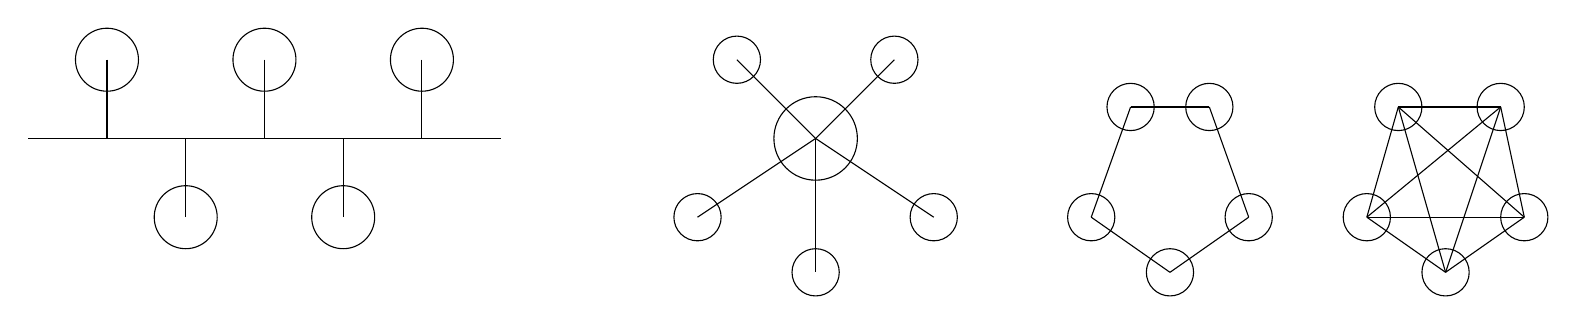
\begin{tikzpicture}
% bus topograpy
\draw (2,-1) circle (\a cm);
\draw (2,-1) -- (2,0);
\draw (4,-1) circle (\a cm);
\draw (4,-1) -- (4,0);
\draw (1,1) circle (\a cm);
\draw (1,1) -- (1,0);
\draw (3,1) circle (\a cm);
\draw (3,1) -- (3,0);
\draw (5,1) circle (\a cm);
\draw (5,1) -- (5,0);
\draw (0,0) -- (6,0);

% star topograpy
\draw (10,0) -- (8.5,-1);
\draw (8.5,-1) circle(\b cm);

\draw (10,0) -- (11.5,-1);
\draw (11.5,-1) circle(\b cm);

% centro
\draw (10,0) circle(\cr cm);

\draw (10,0) -- (10,-1.7);
\draw (10,-1.7) circle(\b cm);

\draw (10,0) -- (9,1);
\draw (9,1) circle(\b cm);

\draw (10,0) -- (11,1);
\draw (11,1) circle(\b cm);

% Rete ad anallo

\draw (13.5,-1) circle(\b cm);
\draw (13.5,-1) -- (14.5,-1.7);
\draw (13.5,-1) -- (14,0.4);

\draw (15.5,-1) circle(\b cm);
\draw (14.5,-1.7) -- (15.5,-1);

\draw (14.5,-1.7) circle(\b cm);
\draw (15.5,-1) -- (15,0.4); 

\draw (14,0.4) circle(\b cm);

\draw (15,0.4) circle(\b cm);
\draw (14,0.4) --  (15,0.4);

% modello a maglia
\draw (17,-1) circle(\b cm);
\draw (19,-1) circle(\b cm);
\draw (17,-1) -- (19,-1);

\draw (17,-1) -- (18,-1.7);
\draw (18,-1.7) circle(\b cm);
\draw (18,-1.7) -- (19,-1);

\draw (18,-1.7) -- (17.4,0.4); 
\draw (17.4,0.4) circle(\b cm);
\draw (17,-1) -- (17.4,0.4);
\draw (17.4,0.4) -- (19,-1);

\draw (18.7,0.4) circle(\b cm);
\draw (18,-1.7) -- (18.7,0.4);
\draw (17,-1) -- (18.7,0.4);
\draw (17.4,0.4) -- (18.7,0.4);
\draw (19,-1) -- (18.7,0.4);
\end{tikzpicture}}
  \caption{Topologie a bus, a stella, ad anello e a maglie}
  \label{fig:topologiepiùutilizzate}
\end{figure}
\begin{oss}
  La topologia a bus era la prima topologia prevista per lo standard TCP/IP,
  infatti, funzionava tramite cavo coassiale cablato direttamente da una scheda
  di rete all'altra, questo sistema non sopravvisse a lungo per il semplice
  motivo che era poco efficente ma soprattutto il coassiale è un cavo semirigido
  e facilmente incline alla rottura, per non parlare dei connettori che hanno
  una tenuto non solida come gli attuali RJ45 e RJ14 per le linee telefoniche,
  come molti standard di questo tipo vengono dritti dal Bell Labs di AT\&T.
\end{oss}

\subsubsection{I significato}
\label{sec:significato}
\begin{defi}
  Il nodo è il mezzo di scambio tra due o più rami, o terminazione degli stessi,
  in questa categori fanno parte sia le terminazioni fisiche di rete che
  gli apparati di comunicazione.
\end{defi}
\begin{defi}
  Il ramo per definizione è il percorso diretto che l'informazione segue per essere
  trasferita tra due nodi, in questa categoria rientrano sia il mezzo trasmissivo che
  la giunzioni fisica/lagica tra due apparati di rete. 
\end{defi}

\subsubsection{Nodi intermedi e terminali}
\label{sec:nodiintermedi}
Il nodo intermedio (\texttt{nodo di commutazione o ralay})
\begin{itemize}
\item Il nodo di scambio, modulazione/demultiplazione;
\item A seconda dei casi viene chiamato Gateway, router, switch, digital cross
  connector, hub, repeater, etc.
\item Concetto simile a quello di parcheggio scambiatore.
\end{itemize}
Nodi terminali ({\it end system})
\begin{itemize}
\item I sorgente/destinazione della comunicazione;
\item Il mezzo attraverso cui un utente usufruisce di uno o più servizi di
  telecomunicazione;
\item Ia variazione di forma: TV, telefono fisso/mobile, PC, elettrodomestici
\end{itemize}
A seconda del livello di astrazione, un nodo può assumere una funzione o l'altra.

\subsection{Definizione di grafo}
\begin{defi}
  I grafi sono struttura matematiche discrete che rivestono interesse sia per la
  matematica che per un'ampia gamma di campi applicativi. In ambito matematico il loro
  studio, la teoria dei grafi, costituisce un'importante parte della combinatoria; i
  grafi inoltre sono utilizzati in aree come topologia, teoria degli automi, funzioni
  speciali, geometria dei poliedri, algebre di Lie. I grafi si incontrano in vari
  capitoli dell'informatica (ad esempio per schematizzare programmi, circuiti, reti di
  computer, mappe di siti). Essi inoltre sono alla base di modelli di sistemi e
  processi studiati nell'ingegneria, nella chimica, nella biologia molecolare, nella
  ricerca operativa, nella organizzazione aziendale, nella geografia (sistemi fluviali,
  reti stradali, trasporti), nella linguistica strutturale, nella storia
  ({\bf alberi genealogici, filologia dei testi})\footnote{\href{https://it.wikipedia.org/wiki/Grafo}{https://it.wikipedia.org/wiki/Grafo}}. 
\end{defi}
\label{sec:grafo}
\begin{figure}[ht]
  \centering
  \def\b{.3}
\def\cr{.53}
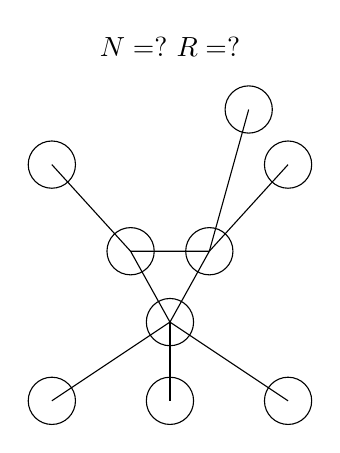
\begin{tikzpicture} 
%\draw (1.5,1.5) circle [radius=\cr];
\node at (1.5,4.5) {$N= ?$ $R=?$};
% centro a maglia
\draw (1.5,1) circle [radius=\b];
\draw (1,1.9) circle [radius=\b];
\draw (2,1.9) circle [radius=\b];
\draw (2,1.9) -- (1,1.9) -- (1.5,1) -- (2,1.9);
% end centro 

\draw (1.5,1) -- (0,0);
\draw (0,0) circle [radius=\b];

\draw (1.5,1) -- (1.5,0);
\draw (1.5,0) circle [radius=\b];

\draw (3,0) -- (1.5,1);
\draw (3,0) circle [radius=\b];

\draw (1,1.9) -- (0,3);
\draw (0,3) circle [radius=\b];

\draw (2,1.9) -- (3,3);
\draw (3,3) circle [radius=\b];

\draw (2,1.9) -- (2.5,3.7);
\draw (2.5,3.7) circle [radius=\b];
\end{tikzpicture}
  \caption{esempio di grafo}
  \label{fig:grafolesempio}
\end{figure}
\begin{itemize}
\item Per definire il Grafo si utilizza la formula:
  \begin{equation}
    \label{eq:grafodef}
    G=(V,A)
  \end{equation}
\item Insieme dei nodi (vertici)
  \begin{equation}
    \label{eq:insiemedeinodi}
    V\text{ con } N=\abs{V}
  \end{equation}
\item Insieme dei rami (archi)
  \begin{equation}
    \label{eq:insiemedeirami}
    A\text{ con } R=\abs{A}
  \end{equation}
\item Grafo orientato: si fa distinzione sul verso di percorrenza dei rami
\end{itemize}
\subsection{Topologie}
\label{sec:top}
Come descritto nel paragrafo esistono differenti topologie, nati per esigenze diverse e
anche in contesti diversi, con peculiarità relative alla costituzione fisica e logica
delle suddette e anche con formule matematiche adite a calcolare eventuali nodi massimi,
la portata della banda passante, etc.  

\subsection{Topologia Elementari}
\label{sec:topologieelementari}
Topologie lineari semplici
\begin{itemize}
\item Ciascun nodo è collegato a due nodi adiacenti con un solo ramo
\end{itemize}
Topologie lineari complesse (\texttt{a struttura gerarchica})
\begin{itemize}
\item Per ogni coppia di nodi esiste un solo percorso di collegamento
\item Ogni nodo è collegato con uno o più rami ai nodi di gerarchia inferiore
\end{itemize}
Topologie magliate
\begin{itemize}
\item Ogni nodo è connesso direttamente agli altri nodi, usando per ciascun
  collegamento un ramo dedicato
\end{itemize}
Topologie a bas
\begin{itemize}
\item Tutti i nodi condividono lo stesso unico collegamento
\end{itemize}

\subsubsection{Topologia a maglia completa}
\label{sec:topologiaamagliacompleta}
In questa topologia ogni nodo è collegato a tutti gli altri presenti, per questo motivo
ha un alta tolleranza ai guasti ma il grosso difetto è l'elevato numero di nodi e quindi
anche i conosti di mantenimento e di realizzazione.
\begin{figure}[ht]
  \centering
  \def\a{.4}
\def\b{.3}
\def\cr{.53}

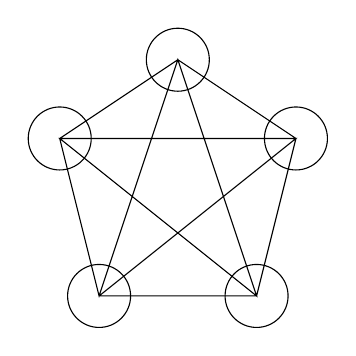
\begin{tikzpicture} 
\draw (0,0) circle [radius=\a];
\draw (0,0) -- (2,0) -- (2.5,2) -- (1,3) -- (-0.5,2) -- (0,0) -- (1,3) -- (2,0) -- (-0.5,2) -- (2.5,2) -- (0,0);
\draw (2,0) circle [radius=\a];
\draw (2.5,2) circle [radius=\a];
\draw (-0.5,2) circle [radius=\a];
\draw (1,3) circle [radius=\a];
\end{tikzpicture}
  \caption{Esempio di topologia a maglia}
  \label{fig:topologiaamagliacompleta}
\end{figure}
\begin{oss}
  Per le sue caratteristiche questa topologia è utilizzata dagli ISP per i collegamenti
  stradali, infatti, per evitare che un'intera zona resti senza servizio solo perché
  un cavo si è rotto il metodo migliore risulta proprio il creare più di una strada
  per portare l'informazione, infatti, come precedentemente spiegato nei capitoli
  precedenti la topoligia davvero utilizzata in molti casi è ibrida.
\end{oss}
\begin{equation}
  \label{eq:magliacompleta}
  R=\sum\limits_{i=1}^N (N-i)=\sum\limits_{i=1}^N N - \sum\limits_{i=1}^N i = N^2-
  \frac{N(N+1)}{2} = \frac{N(N-1)}{2}
\end{equation}